\chapter{Análisis}
% Planeacion del sistema
% Siguiente capitulo: Primer prototipo - Desarrollo Frontend
%   - Analisis
%   - Diseno
%   - etc...

\section{Alcance}

La magnitud de este problema abarca a todos los organismos, direcciones o cualquier dependencia del Instituto Politécnico Nacional. Aunque la solución puede escalar a todo el instituto y su marco normativo, el alcance de este proyecto \textit{considerará únicamente a la comunidad de la Escuela Superior de Cómputo y a los reglamentos con mayor relevancia para las actividades académicas}. Para ello, en este proyecto, inicialmente contará con los siguientes 

\begin{itemize}
    \item Ley Orgánica
    \item Reglamento Interno
    \item Reglamento de Titulación
    \item Reglamento General de Estudios
\end{itemize}

\section{Requerimientos Funcionales}

A continuación, se describe el comportamiento y la funcionalidad esencial para que el chatbot pueda cumplir el objetivo:

\begin{enumerate}[leftmargin=2.5cm ,label={\bfseries RF-\arabic*}]
    \item \label{itm:consultar-reglamento} Un usuario de esta aplicación debe poder consultar un segmento de los documentos del marco normativo en cualquiera de los siguientes niveles de división estructural del documento:
    \begin{itemize}
        \item título
        \item capítulo
        \item sección
        \item artículo.
    \end{itemize}
    
    \item La aplicación debe manejar una conversación de manera lógica (i.e., responder adecuadamente a la conversación en los temas a las preguntas referentes al marco normativo).
    \item \label{itm:requisito-intenciones} El chatbot debe poder detectar si la intención del mensaje es alguno de los siguientes:
        \begin{itemize}
            \item Saludar.
            \item Solicitar información de un articulo.
            \item Solicitar artículos relacionados a una situación en particular.
            \item Despedir.
        \end{itemize}
    \item El chatbot debe saludar de acuerdo a la hora del día.
    \item El chatbot debe poder identificar las entidades o conceptos que el usuario solicita consultar.
    \item \label{itm:rf-servicio-web} La aplicación debe ser disponible a través de un servicio web.
    \item  \label{itm:cliente-web} La aplicación debe proporcionar un cliente accesible a través de un navegador web.
\end{enumerate}

\section{Requerimientos No Funcionales}

\begin{enumerate}[leftmargin=2.5cm ,label={\bfseries RNF-\arabic*}]
    \item Se sugiere que el resultado de las consultas sean breves y concisos. 
    \item El bot debe poder expresar intenciones de asesorar en temas referentes al marco normativo.
    \item Se desea que la aplicacion se desarrolle utilizando herramientas de licencia abierta y software libre.
\end{enumerate}

\section{Metodología}

Las actividades a desarrollarse se harán siguiendo una metodología de \textbf{prototipado evolutivo}. Esta elección se hace con base a la necesidad de estar evaluando constantemente el diseño inicial y los ajustes en la implementación. Los prototipos están basado en los siguientes tres componentes:

\begin{itemize}
    \item \textbf{Interfaz de usuario}: contiene la página web y el sistema cliente que se encarga de realizar peticiones HTTP al chatbot.
    \item \textbf{Base de conocimiento}: serialización y persistencia del conocimiento de los documentos normativos y su representación semántica necesaria para poder procesarla.
    \item \textbf{Intérprete semántico}: componente de entendimiento del chatbot que se encarga de procesar consultas textuales en búsquedas de similitud sobre la base de conocimiento.
\end{itemize}

Con base a estos componentes, se definen los siguientes prototipos:

\subsection{Primer Prototipo}

En este primer prototipo inicial se espera construir el componente gráfico del sistema cliente así como la implementación del modelo de datos para la base de conocimiento. Las funcionalidades de este prototipo son:

\begin{itemize}
    \item Construcción de la página web
    \item Desarrollo del sistema cliente
    \item Construcción del modelo de datos inicial
\end{itemize}

\subsection{Segundo Prototipo}

En este segunda iteración del prototipado se enfocará principalmente a conectar los componentes y un flujo general funcionando para la atención de consultas. Las funcionalidades adicionales a la primera iteración serán:

\begin{itemize}
    \item Transformación semántica de texto
    \item Ejecución del algoritmo de similitud.
    \item Recuperación de artículos de la base de datos.
\end{itemize}


Así 
% \begin{figure}
%     \centering
%     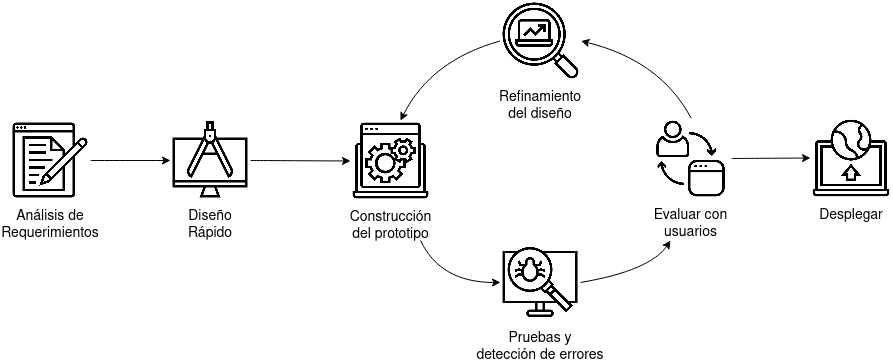
\includegraphics[scale=0.47]{images/6/prototipado_evolutivo}
%     \caption{Ciclo de vida del proyecto}
%     \label{fig:ciclo-vida-metodologia}
% \end{figure}

\subsection{Tercer Prototipo}

En la última iteración del proyecto 

\section{Cronograma de Actividades}

\begin{figure}[ht]
    \centering
    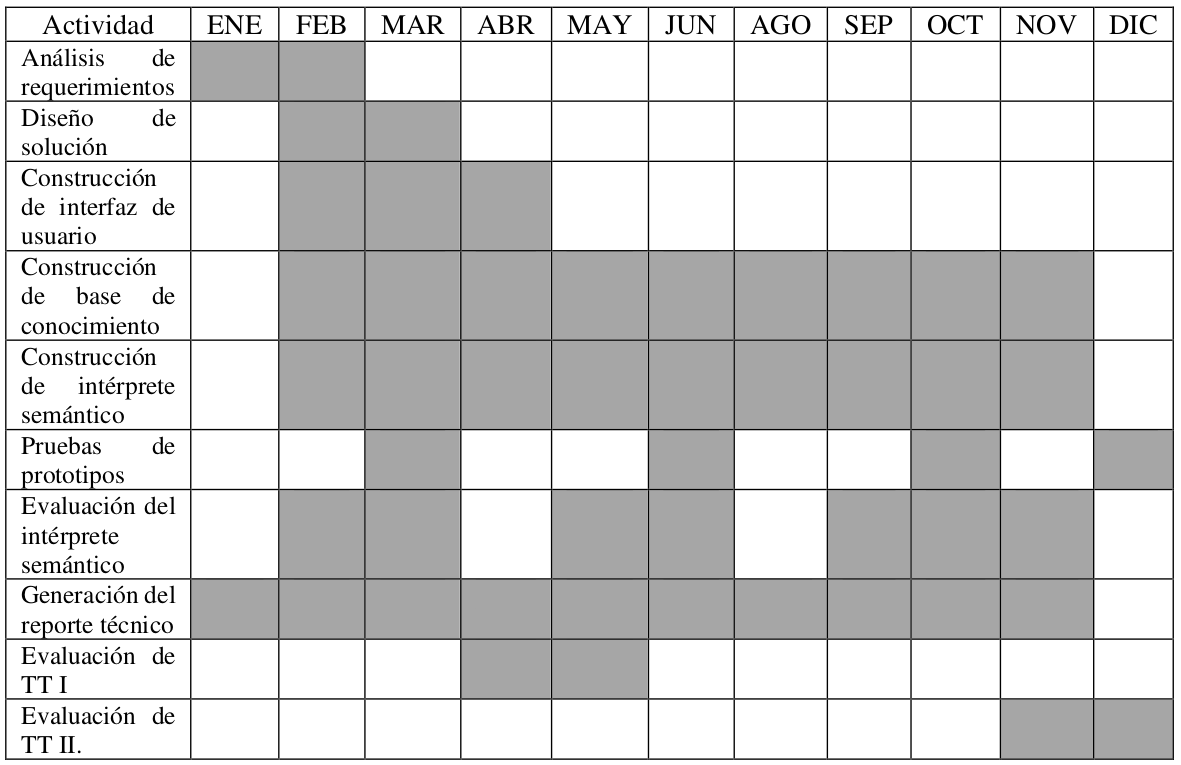
\includegraphics[scale=0.38]{images/6/cronograma}
    \caption{Cronograma de actividades para el desarrollo de este proyecto.}
    \label{fig:cronograma}
\end{figure}
